\documentclass{article}
\usepackage{tikz}

\usetikzlibrary{angles}
\input code-with-output
\begin{document}

\begin{example*}{Markup a right angle}
  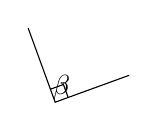
\begin{tikzpicture}
    \draw (20:1cm) coordinate (A) -- (0, 0) coordinate (O) -- (110:1cm) coordinate (B) 
      pic [draw, pic text=$\beta$, angle radius=5pt, angle eccentricity=.8] {right angle = A--O--B};
  \end{tikzpicture}
\end{example*}

\verb|angle radius = \i, angle eccentricity = \j|\par

\foreach \i in {5pt, 10pt, 15pt} {
  \texttt{\textbackslash i = \i}:
  \foreach \j in {0.5, 1, 1.5} {
    \rlap{\begin{tikzpicture}[baseline=(text.base)]
      \draw (20:1cm) coordinate (A) -- (0, 0) coordinate (O) -- (110:1cm) coordinate (B);
      \pic [draw, pic text=$\beta$, angle radius=\i, angle eccentricity=\j] {right angle = A--O--B};
      \node (text) at (.3, -.3) {\texttt{\textbackslash j = \j}};
    \end{tikzpicture}}\hspace*{50pt}
  }\par
}

\end{document}